\section{Assumptions}

This thesis proposes the existence of high-level musical concepts, including melody, harmony, rhythm, form, motif, and counterpoint. These concepts, despite changes in sonic qualities, demonstrate enduring independence. Additionally, these elements are interactive, continually evolving within the musical context. This echoes the nature of the symbolic domain, such as sheet music, which retains its essence despite varied interpretations across diverse performances, instruments, and styles. While a single waveform might correspond to a finite set of sheet music representations encapsulating its musical components, one piece of music can be interpreted infinitely, varying by instruments, voices, tempos, and performance styles.

Abstract high-level features can be discerned irrespective of the waveform or production style, providing an objective, comprehensive insight into the musical content of a composition. This approach is akin to analyzing sheet music to uncover its foundational behaviors.

These features enable listeners to identify and recreate musical structures by ear, fostering deeper engagement with music. Heuristics, mental shortcuts, or rules of thumb facilitate rapid comprehension of complex musical concepts, bringing underlying patterns and structures into focus.

For example, despite differences in cultural contexts, stylistic elements, time signatures, key signatures, and sonic properties, we propose a similarity between figures \ref{fig:mahler} and \ref{fig:giant_steps}. Both pieces exhibit the same musicological fingerprint, so to speak, derived from the envelope of their melodic and harmonic contours through non-diatonic major thirds.

This concept aligns with the theories of Kurt Koffka, a founding member of the Gestalt school of psychology, who advocated for a holistic approach to understanding complex forms, as opposed to the structuralist practice of dissecting mental processes into their elemental components \cite{Koffka2013PrinciplesPsychology}. In the context of music, Gestalt psychology principles suggest our minds process auditory input similarly to visual input, by seeking patterns and structures. This understanding significantly enhances the comprehension of cognitive processes in musical perception and organization, influencing music theory, cognition, and therapy \cite{Lerdahl1985AMusic}.

\begin{figure}[ht]
    \centering
    \scalebox{0.9}{
    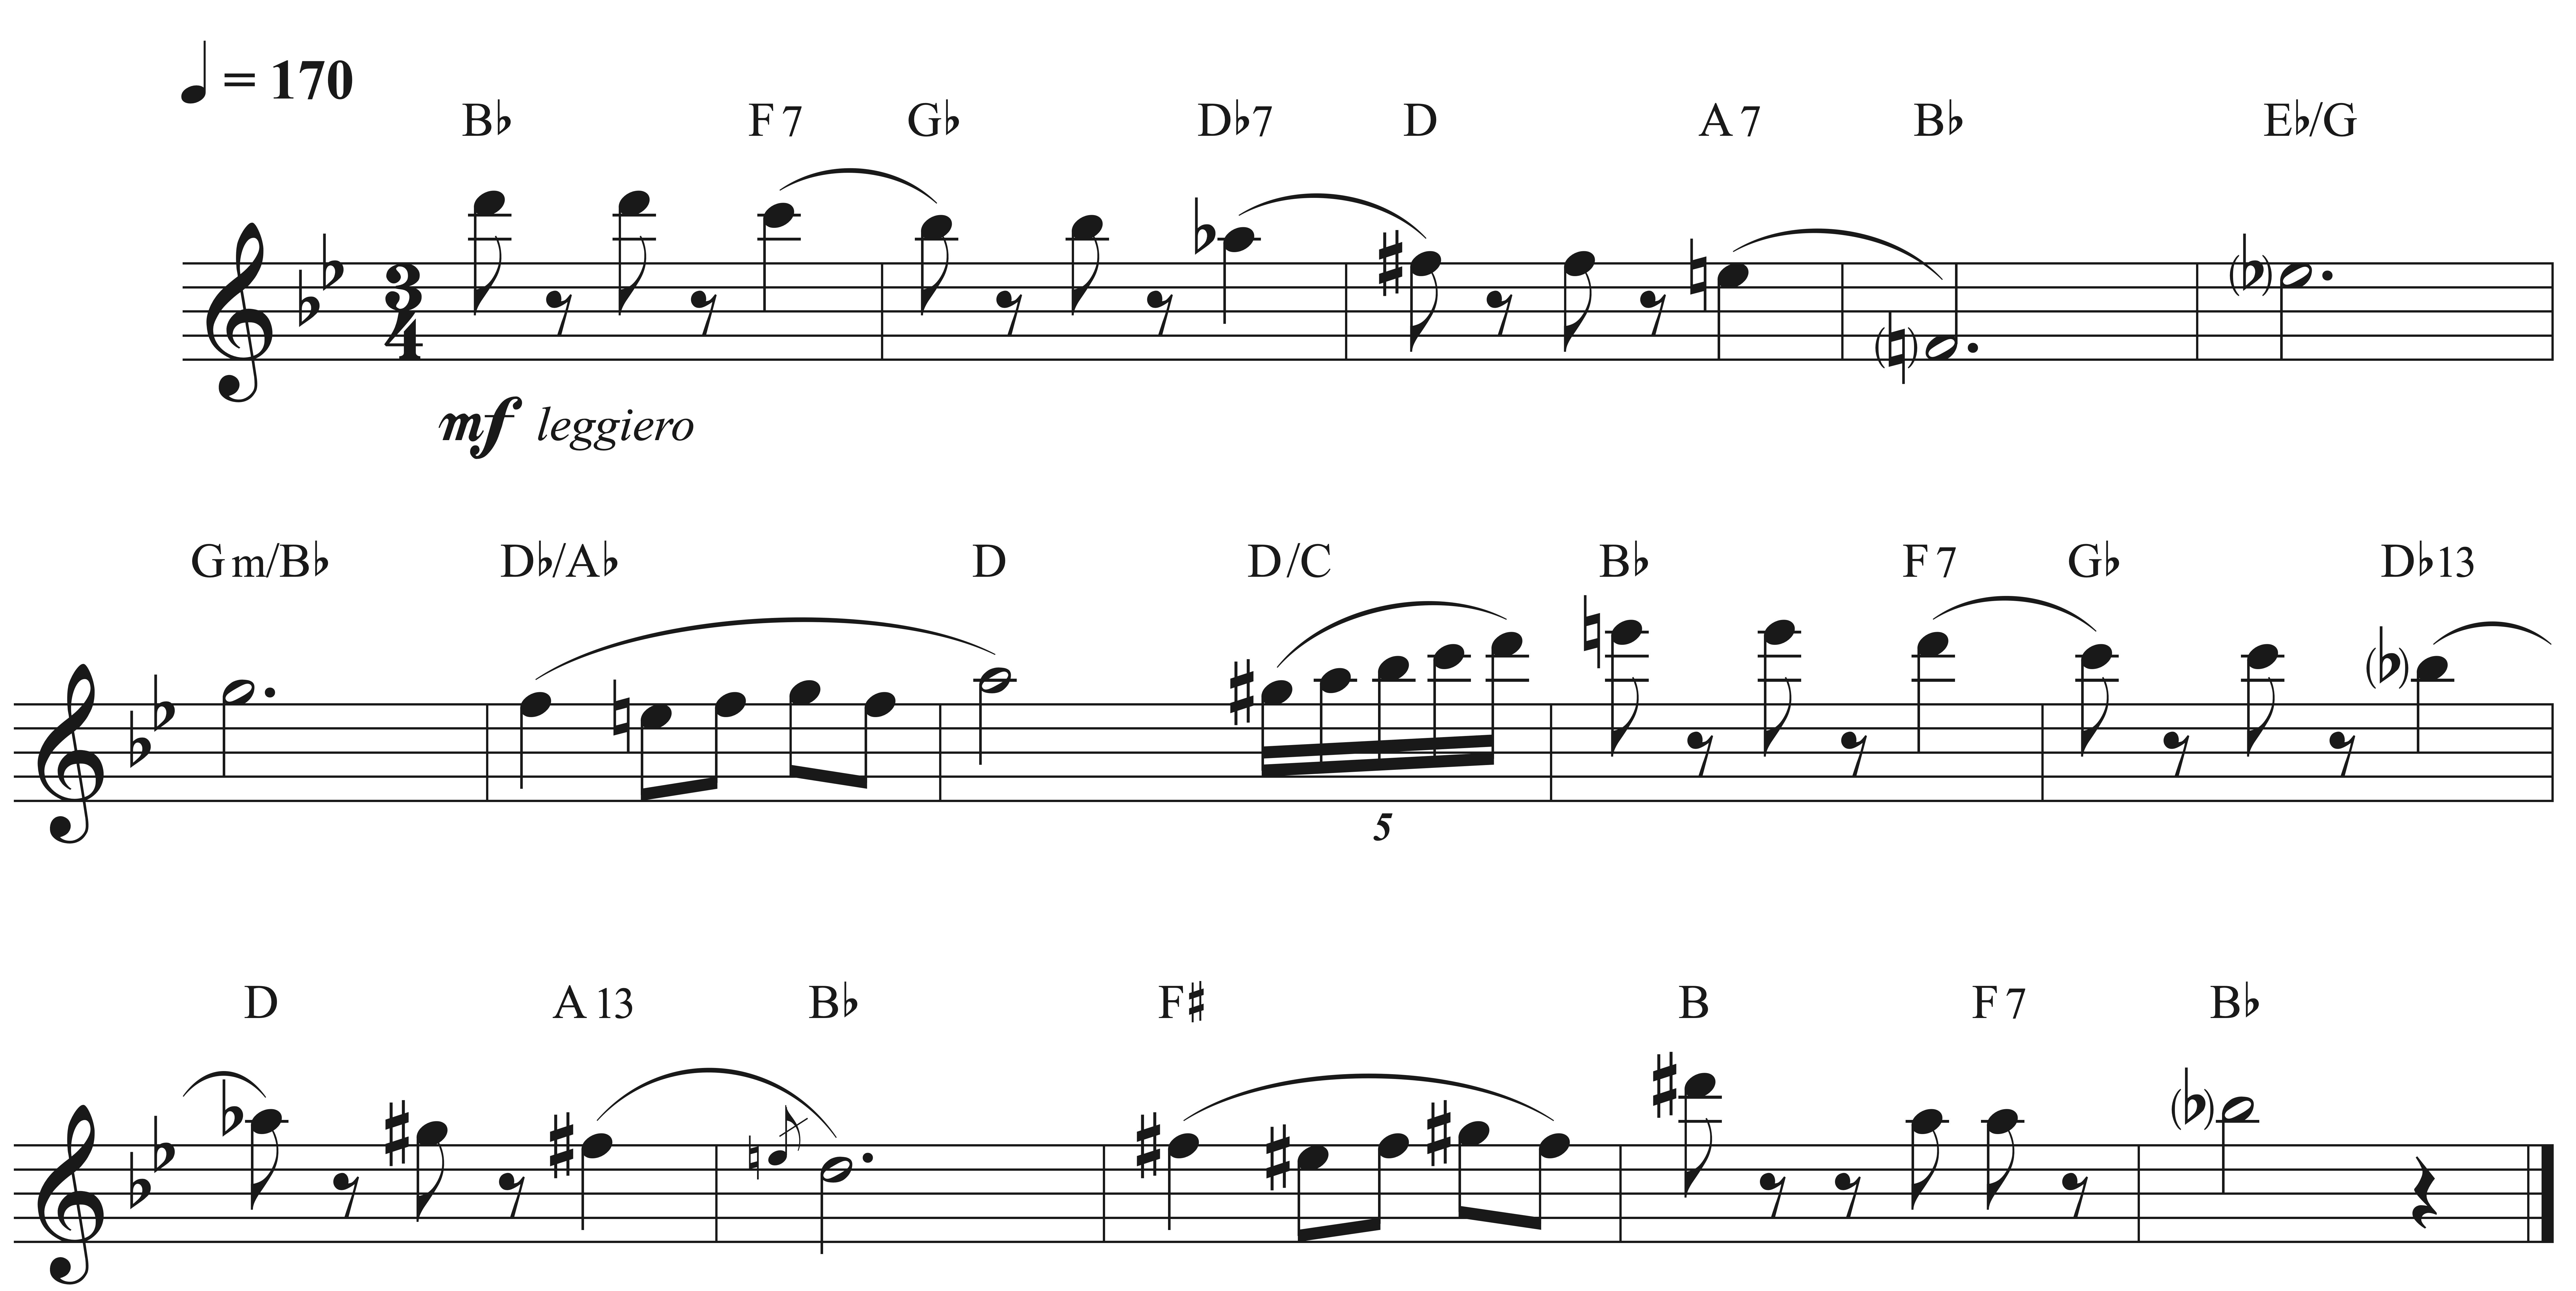
\includegraphics[width=\textwidth]{figures/images/Mahler 9 Giant Steps score.png}
        }
    \caption[Mahler's 9th Symphony, 2nd movement]{\small{A small excerpt from Mahler's 9th Symphony, 2nd movement: The melodic and harmonic contour propels through non-diatonic major thirds.}}
    \label{fig:mahler}
\end{figure}

\begin{figure}[ht]
    \centering
    \scalebox{0.9}{
    \includegraphics[width=\textwidth]{figures/images/giant steps score.png}
        }
    \caption[Giant Steps]{\small{John Coltrane's Giant Steps head: A testament to harmonic exploration, featuring rapid chord changes in non-diatonic major thirds.}}
    \label{fig:giant_steps}
\end{figure}
